Understanding complex visual environments from egocentric video is a fundamental challenge in computer vision, requiring persistent memory of observed scenes, structured spatial reasoning, and efficient processing of long video sequences.
Recent advances in vision-language models~\cite{kaduri2025s, liu2025survey, comanici2025gemini, bai2025qwen2} have enabled remarkable scene understanding capabilities, yet these models face inherent limitations: they lack persistent, structured scene memory; their reasoning over spatial relationships remains implicit and unexplainable; and their computational cost scales poorly with video duration.

We introduce VL-KnG (Vision-Language Knowledge Graph), a training-free framework that addresses these limitations by constructing \textit{persistent spatiotemporal knowledge graphs} from egocentric video and enabling structured reasoning through graph-based retrieval-augmented generation (GraphRAG)~\cite{Han2024RetrievalAugmentedGW}.
As depicted in \Cref{fig:real_world_grid}, VL-KnG is deployed in a real-world navigation scenario, where the system answers natural language queries over the constructed graph and localizes the relevant goal object in the video stream.

Our \textit{key insight} is that explicit structured scene representations provide complementary advantages to direct VLM inference—particularly in explainability~\cite{tiddi2022knowledge}, computational efficiency, and adaptability across diverse downstream tasks. 
Crucially, direct VLM inference requires re-processing all sampled frames for every new query, causing the computational cost to grow as $O(\text{queries} \times \text{frames})$. 
In contrast, \textit{VL-KnG processes the video once with cost $O(\text{frames})$ to construct a persistent spatiotemporal knowledge graph}, after which queries can be answered efficiently via lightweight subgraph retrieval without re-ingesting any video frames. 
The retrieved subgraph also provides a structured and inspectable reasoning trace, in contrast to the opaque end-to-end reasoning of VLMs.

From a representation perspective, prior approaches typically fall into two categories. 
Fine-grained scene graphs~\cite{3dgraphllm2025iccv, fross2025iccv} capture detailed object-level semantics but are usually local and often rely on 3D reconstruction, while topological graphs~\cite{chiang2024mobility, gsavln2025iclr} model large environments but lack rich object-level semantics. 
\textit{VL-KnG unifies these paradigms by constructing spatiotemporal knowledge graphs that preserve object-level detail and rich spatial relationships while scaling to large environments from monocular video}, with persistent object identity maintained across temporal sequences.
\begin{figure*}[t]
    \centering
    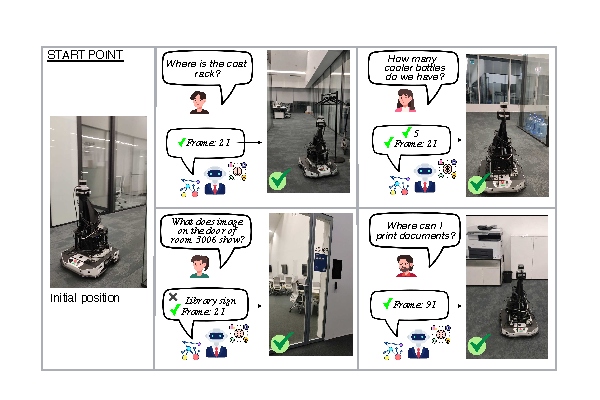
\includegraphics[width=0.9\linewidth]{Figs/navigation_eccv.pdf}
    \caption{Real-world deployment examples of VL-KnG for embodied scene understanding. The system processes natural language queries over a spatiotemporal knowledge graph to identify relevant objects and provide frame-level localization, enabling downstream tasks such as navigation goal identification.}
    \label{fig:real_world_grid}
\end{figure*}
VL-KnG processes video sequences in chunks using modern VLMs~\cite{comanici2025gemini, bai2025qwen2}, constructing a spatiotemporal knowledge graph that maintains object identity across time via LLM-based Spatiotemporal Object Association (STOA), while capturing rich semantic and spatial relationships.
The system employs GraphRAG-based query processing~\cite{Han2024RetrievalAugmentedGW} for efficient subgraph retrieval and reasoning.
We further extend the pipeline with Graph-Enhanced Retrieval (GER), which augments graph-based retrieval with SigLIP2-based \cite{tschannen2025siglip} visual grounding for improved frame localization.

We evaluate VL-KnG on three benchmarks spanning diverse environments:
\textbf{OpenEQA}~\cite{majumdar2024openeqa} (1,636 embodied QA pairs across 180+ indoor environments),
\textbf{NaVQA}~\cite{anwar2024remembr} (descriptive QA over indoor/outdoor driving sequences), and
\textbf{WalkieKnowledge}, our new proposed benchmark with approximately 200 manually annotated questions across 8 egocentric trajectories.
Our contributions are:
\begin{itemize}
\item \textbf{A training-free pipeline for constructing spatiotemporal knowledge graphs from monocular video}, using VLM-based detection~\cite{comanici2025gemini} and LLM-based Spatiotemporal Object Association (STOA) to maintain persistent object identity---without 3D reconstruction, depth sensing, or task-specific training.
\item \textbf{Graph-Enhanced Retrieval (GER)}---a hybrid approach combining Graph\-RAG~\cite{Han2024RetrievalAugmentedGW} subgraph retrieval with SigLIP2~\cite{tschannen2025siglip} visual grounding for improved frame localization.
\item \textbf{WalkieKnowledge benchmark} with approximately 200 annotated questions across 8 diverse egocentric trajectories enabling comparison between structured approaches and general-purpose VLMs.
\end{itemize}
